\subsection{introduction}
	\begin{frame}{denoising}{introduction}
		\begin{itemize}
			\item	\textbf{problem}: signal $y$ is noisy
                \begin{equation*}
                    y(i) = x(i) + n(i)                    
                \end{equation*}
            \pause
            \item   \textbf{assumptions}:
                \begin{itemize}
                    \item   noise is uncorrelated
                    \item   noise is stationary
                \end{itemize}
            \pause
            \smallskip \item   \textbf{objective}: estimate $\hat{x}$ which minimizes the error
                \begin{equation*}
                    e(i)  = x(i) - \hat{x}(i)
                \end{equation*}
            \pause
            \item   \textbf{approach}: filter the noisy signal
                \begin{equation*}
                    \hat{x}(i) = \sum\limits_{j=0}^{\mathcal{O}-1} w(j)\cdot y(i-j)
                \end{equation*}
		\end{itemize}
	\end{frame}
    \begin{frame}{denoising}{introduction 2/2}
        here: only presenting the simplest approach to noise reduction
        
        
        \pause
        \bigskip
        the \textbf{Wiener Filter}
	\end{frame}

\subsection{Wiener Filter}
	\begin{frame}{denoising}{Wiener filter 1/2}
        \begin{footnotesize}
        \begin{eqnarray*}
            \hat{x}(i) &=& \sum\limits_{j=0}^{\mathcal{O}-1} w(j)\cdot y(i-j)\\
            %\vec{\hat{x}} &=& \vec{w}^T\vec{y}\\   
            \pause
            \hat{X}(\jom) &=& W(\jom)\cdot Y(\jom)\\
            E(\jom) &=& X(\jom) - W(\jom)\cdot Y(\jom)
        \end{eqnarray*}
            \pause
            \bigskip
        \begin{eqnarray*}
            \frac{\partial \mathcal{E}\lbrace |E(\jom)|^2\rbrace}{\partial W(\jom)} &=& 0\\
            \frac{\partial \mathcal{E}\lbrace (X(\jom) - W(\jom)\cdot Y(\jom))^*(X(\jom) - W(\jom)\cdot Y(\jom))\rbrace}{\partial W(\jom)} &=& 0\\
            2W(\jom)S_\mathrm{YY}(\jom) - 2S_\mathrm{XY}(\jom) &=&0\\
            \pause
            \bigskip\Rightarrow
            W(\jom) &=& \frac{S_\mathrm{XY}(\jom)}{S_\mathrm{YY}(\jom)}
        \end{eqnarray*}
        \end{footnotesize}
 	\end{frame}

	\begin{frame}{denoising}{Wiener filter 2/2}
       reminder: signal and noise are uncorrelated $\rightarrow r_\mathrm{XN}(i) = 0$
        \begin{eqnarray*}
            \mat{R}_\mathrm{YY} &=& \mat{R}_\mathrm{XX} + \mat{R}_\mathrm{NN}\\
            \vec{r}_\mathrm{XY} &=& \vec{r}_\mathrm{XX}\\
            \bigskip
            \pause
            \Rightarrow {S}_\mathrm{YY}(\jom) &=& {S}_\mathrm{XX}(\jom) + {S}_\mathrm{NN}(\jom)\\
            \Rightarrow {S}_\mathrm{XY}(\jom) &=& {S}_\mathrm{XX}(\jom)\\
            \pause
            \bigskip
            \Rightarrow
            W(\jom) &=& \frac{S_\mathrm{XX}(\jom)}{{S}_\mathrm{XX}(\jom) + {S}_\mathrm{NN}(\jom)}\\
            \bigskip
            &=& \frac{S_\mathrm{YY}(\jom) - S_\mathrm{NN}(\jom)}{{S}_\mathrm{YY}(\jom)}
        \end{eqnarray*}
 	\end{frame}

	\begin{frame}{denoising}{Wiener filter discussion 1/2}
 \setbeamercovered{invisible}
      \vspace{-3mm} \begin{eqnarray*}
            W(\jom) &=& \frac{S_\mathrm{XX}(\jom)}{{S}_\mathrm{XX}(\jom) + {S}_\mathrm{NN}(\jom)}\\
            \pause
            &=& \frac{SNR(\omega)}{SNR(\omega) + 1}
        \end{eqnarray*}
        \smallskip
        $\Rightarrow$ attenuates noisy components \textit{in proportion to SNR}
        \begin{figure}
            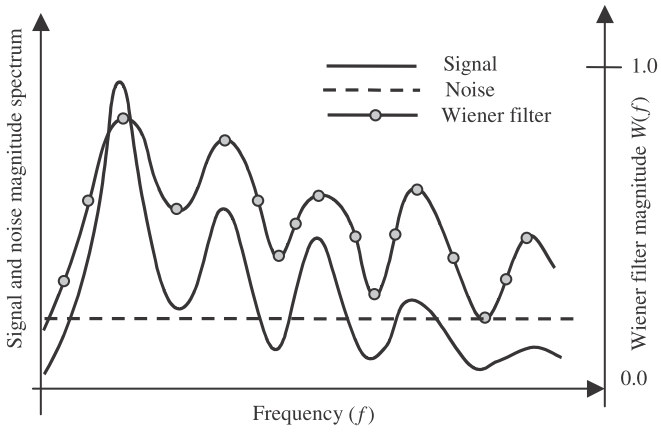
\includegraphics[scale=.4]{graph/Wiener}
        \end{figure}
 	\end{frame}

	\begin{frame}{denoising}{Wiener filter discussion 2/2}
      \vspace{-3mm} \begin{eqnarray*}
            W(\jom) &=& \frac{S_\mathrm{XX}(\jom)}{{S}_\mathrm{XX}(\jom) + {S}_\mathrm{NN}(\jom)}\\
            \pause
            &=& \frac{SNR(\omega)}{SNR(\omega) + 1}
        \end{eqnarray*}
        \smallskip
        $0\leq W(\jom)\leq 1$
        
        \begin{columns}
        \column{.6\textwidth}
        \begin{itemize}
            \item   limiting case 1: noise free
                \begin{eqnarray*}
                    SNR(\omega) &=& \infty\\
                    \pause
                    \Rightarrow  
                    W(\jom) &\rightarrow & 1
                \end{eqnarray*}
            \item   limiting case 2: extr. noisy
                \begin{eqnarray*}
                    SNR(\omega) &=& 0\\
                    \pause
                    \Rightarrow  
                    W(\jom) &\rightarrow & 0
                \end{eqnarray*}
        \end{itemize}
        \column{.4\textwidth}
        \begin{figure}
            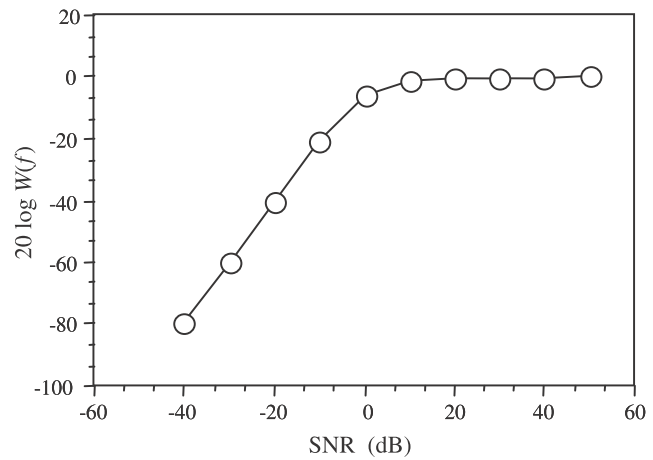
\includegraphics[scale=.3]{graph/WienerSNR}
        \end{figure}
        \end{columns}
 	\end{frame}

	\begin{frame}{denoising}{Wiener filter question}
        How to estimate the noise spectrum?
	\end{frame}

\subsection{Spectral Subtraction}
 \setbeamercovered{invisible}
	\begin{frame}{denoising}{Spectral Subtraction}
        \begin{itemize}
            \item[] \textbf{idea}: Why not subtract the noise spectrum from the signal spectrum?
        \end{itemize}
        \begin{eqnarray*}
            |\hat{X}(\jom)|^2 &=& |Y(\jom)|^2 - |N(\jom)|^2\\
            &=& H(\jom)\cdot |Y(\jom)|^2\\
        \end{eqnarray*}
            \bigskip
            \pause
        \begin{eqnarray*}
            \Rightarrow H &=& 1-\frac{|N(\jom)|^2}{|Y(\jom)|^2}\\
            &=& \frac{|Y(\jom)|^2-|N(\jom)|^2}{|Y(\jom)|^2}
        \end{eqnarray*}
        \pause
        spectral subtraction identical to  Wiener filter when the power density spectrum estimates approach the ensemble means
	\end{frame}
